\documentclass{beamer}
\beamertemplatenavigationsymbolsempty
\usecolortheme{beaver}
\setbeamertemplate{blocks}[rounded=true, shadow=true]
\setbeamertemplate{footline}[page number]
\usefonttheme{professionalfonts}

\title{Bayesian Neural Network Priors Revisited}
\author{Vincent Fortuin et al.}
\institute{Talk by: Fedor Sobolevsky}
\date{}

\begin{document}

\begin{frame}
\titlepage
\end{frame}

\begin{frame}
\frametitle{Main Idea}
\begin{itemize}
    \item \textbf{Problem}: Isotropic Gaussian priors are the de facto standard for Bayesian Neural Networks (BNNs), but may not reflect true beliefs about weight distributions
    \item \textbf{Observation}: Networks trained with SGD show systematic patterns in weight distributions that differ from isotropic Gaussians
    \item \textbf{Hypothesis}: Building these empirical patterns into priors can improve BNN performance
    \item Better priors may help explain/mitigate the "cold posterior effect" (improved performance with tempered posteriors)
\end{itemize}
\end{frame}

\begin{frame}
\frametitle{Current Method: Gaussian Priors}
\begin{itemize}
    \item \textbf{Isotropic Gaussian priors} are used across almost all Bayesian deep learning.
    
    \item \textbf{Advantages}:
    \begin{itemize}
        \item Simple to implement and optimize
        \item Maximum entropy for given variance
        \item Well-studied theoretical properties
    \end{itemize}
    
    \item \textbf{Problems}:
    \begin{itemize}
        \item May not reflect true weight distributions
        \item Can lead to poor predictive performance vs SGD
        \item May contribute to cold posterior effect
    \end{itemize}
\end{itemize}
\end{frame}

\begin{frame}
\frametitle{Empirical Weight Distributions in FCNNs}
\begin{center}
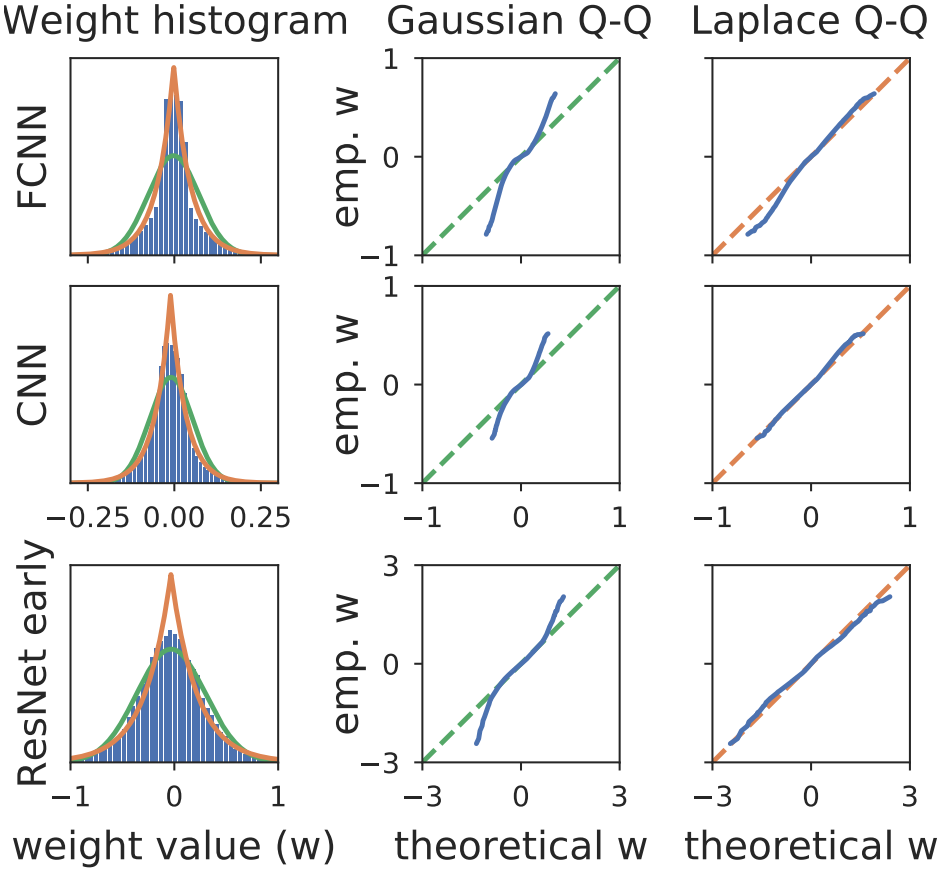
\includegraphics[width=0.8\textwidth]{fcnn_weights.png}
\end{center}
\end{frame}

\begin{frame}
\frametitle{Spatial Correlations in CNN Weights}
\begin{center}
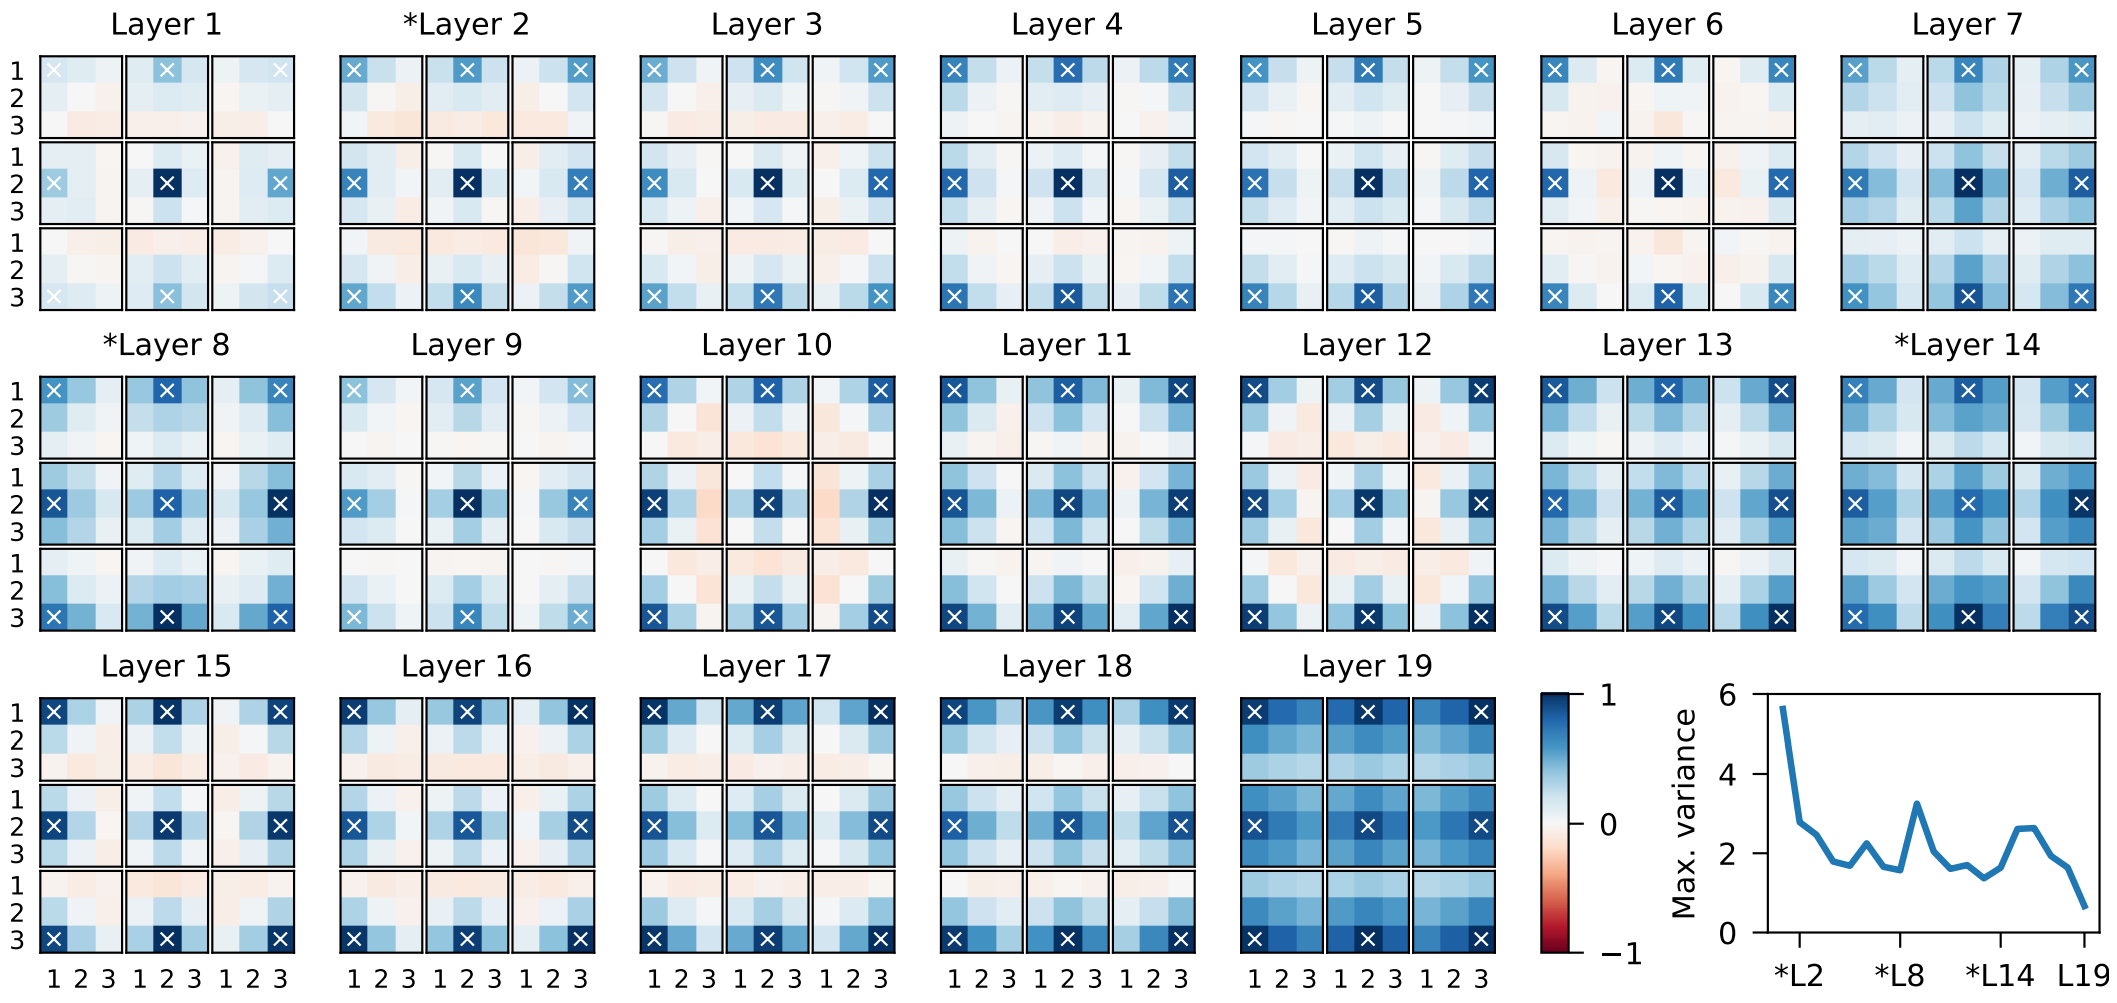
\includegraphics[width=\textwidth]{cnn_correlations.png}
\end{center}
\begin{itemize}
    \item CNN/ResNet weights show \textbf{strong spatial correlations}
    \item Nearby pixels in filters are highly correlated
    \item Correlation strength increases in deeper layers
\end{itemize}
\end{frame}

\begin{frame}
\frametitle{Alternative Prior Distributions}
\begin{itemize}
    \item \textbf{Heavy-tailed priors for FCNNs}:
    \begin{itemize}
        \item Laplace distribution: $p(x) = \frac{1}{2b}\exp\left(-\frac{|x-\mu|}{b}\right)$
        \item Student-t distribution: adjustable tail heaviness via $\nu$ parameter
    \end{itemize}
    
    \item \textbf{Correlated Gaussian priors for CNNs/ResNets}:
    \begin{itemize}
        \item Multivariate Gaussian with block-diagonal covariance
        \item Matern kernel ($\nu=1/2$) for spatial correlations:
        $$\text{cov}(w_{i,j},w_{i',j'}) = \sigma^2\exp\left(\frac{-d(j,j')}{\lambda}\right)$$
    \end{itemize}
\end{itemize}
\end{frame}

\begin{frame}
\frametitle{Performance: FCNNs with Different Priors}
\begin{center}
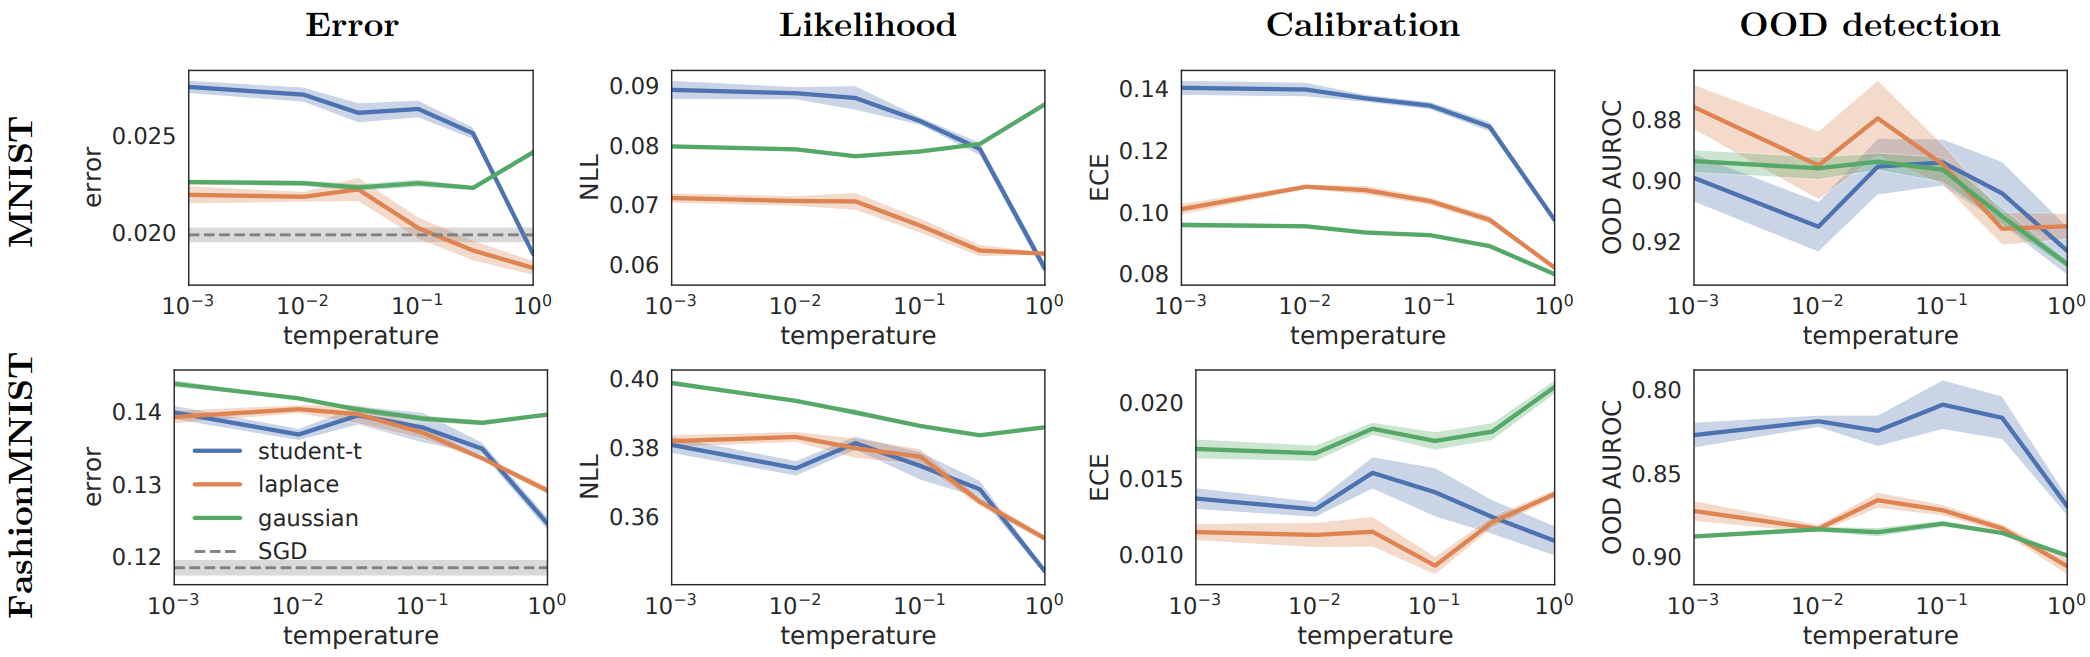
\includegraphics[width=0.9\textwidth]{fcnn_performance.png}
\end{center}
\begin{itemize}
    \item Heavy-tailed priors outperform Gaussian in test error/NLL
    \item Eliminate cold posterior effect in FCNNs
\end{itemize}
\end{frame}

\begin{frame}
\frametitle{Performance: CNNs/ResNets with Different Priors}
\begin{center}
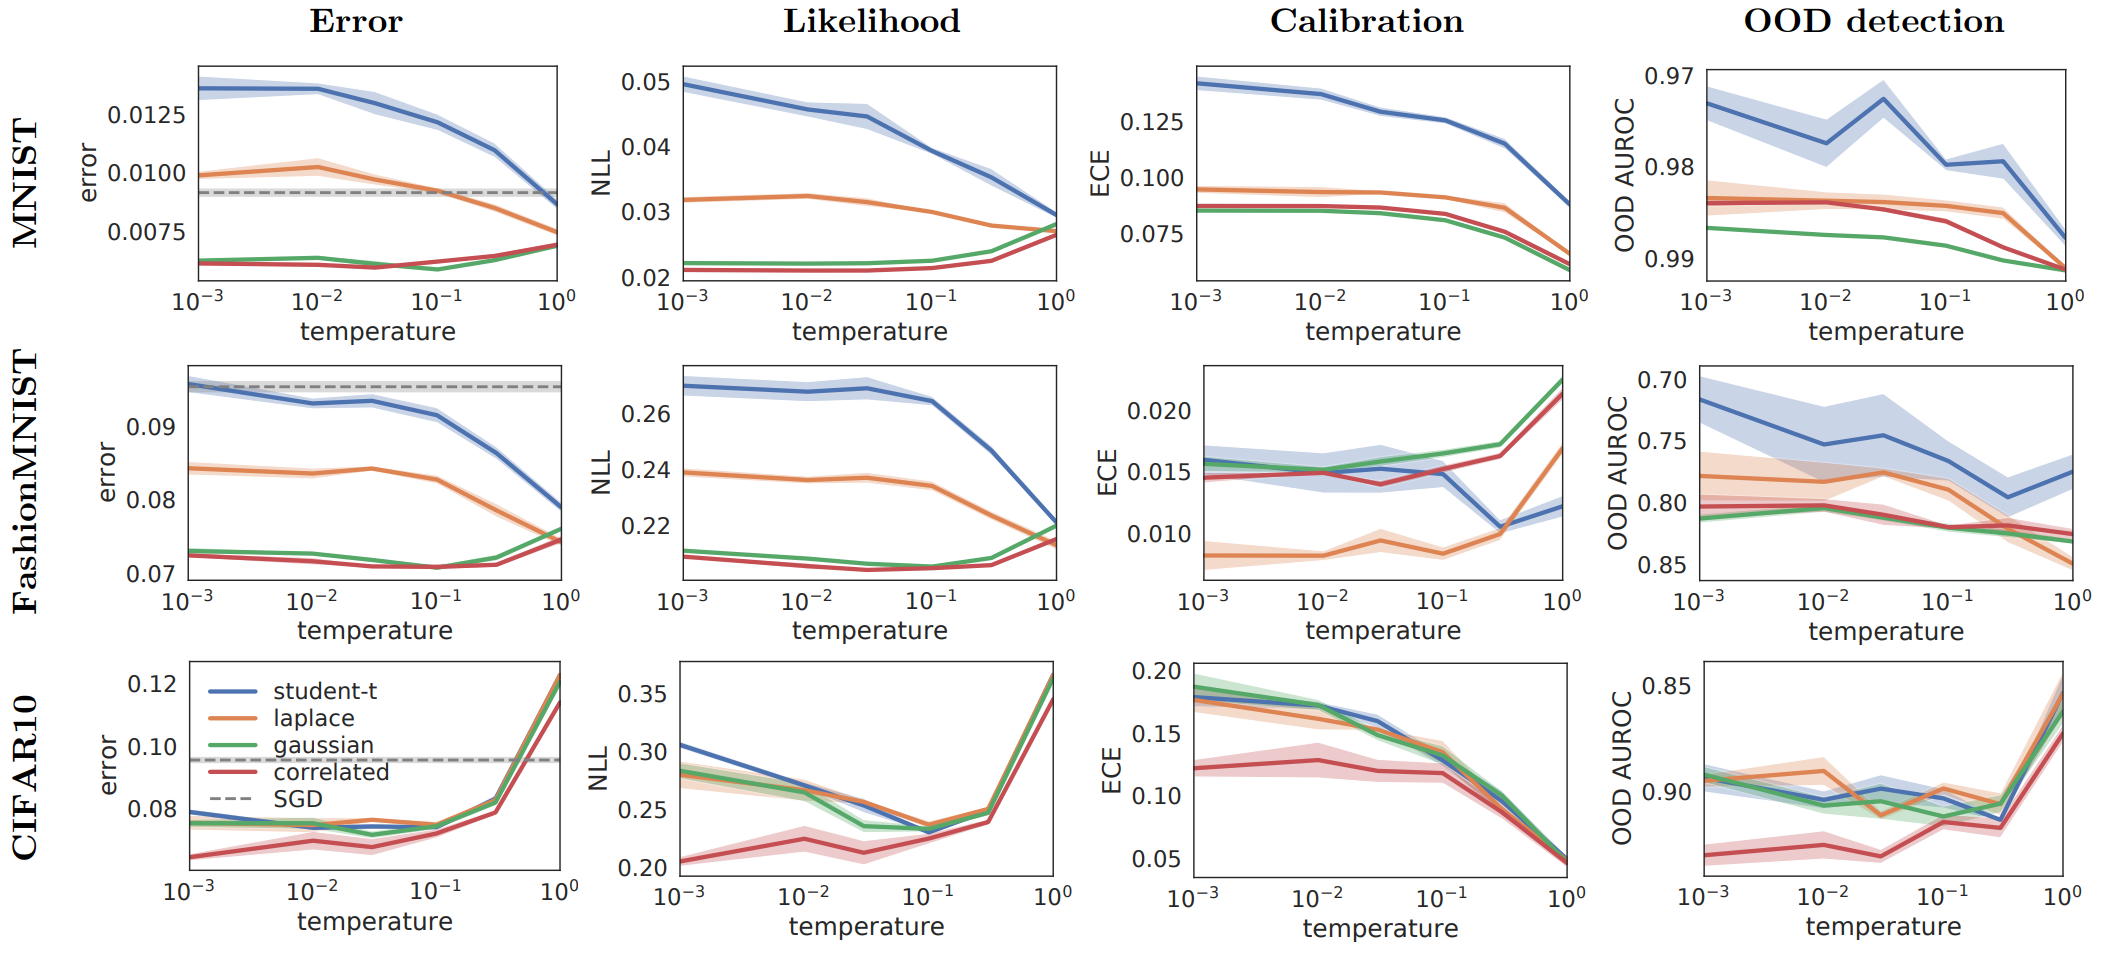
\includegraphics[width=0.9\textwidth]{cnn_performance.png}
\end{center}
\begin{itemize}
    \item Correlated Gaussian priors outperform isotropic ones
    \item Heavy-tailed priors reduce cold posterior effect but hurt performance
    \item Correlated priors \textit{increase} cold posterior effect in ResNets
\end{itemize}
\end{frame}

\begin{frame}
\frametitle{Key Takeaways}
\begin{itemize}
    \item \textbf{Empirical analysis matters}: SGD-trained networks show systematic patterns that should inform prior choice
    \item \textbf{Architecture-dependent priors}:
    \begin{itemize}
        \item FCNNs: Heavy-tailed priors (Laplace/Student-t)
        \item CNNs/ResNets: Spatially correlated Gaussian priors
    \end{itemize}
    
    \item \textbf{Cold posterior effect}:
    \begin{itemize}
        \item In FCNNs: Likely due to prior misspecification (fixed by heavy-tailed priors)
        \item In ResNets: More complex (possibly likelihood/data augmentation issues)
    \end{itemize}
\end{itemize}
\end{frame}

\end{document}